\documentclass[aspectratio=169, 10pt]{beamer}

% --- PACKAGES ---
\usepackage[utf8]{inputenc}
\usepackage{tikz}
\usetikzlibrary{shapes.geometric, arrows.meta, positioning, calc}
\usepackage{booktabs}
\usepackage{array}
\usepackage{xcolor}

% --- COLOR PALETTE ---
\definecolor{Ink}{HTML}{1A1D23}
\definecolor{Dim}{HTML}{6B7280}
\definecolor{Accent}{HTML}{2C5F8A}
\definecolor{AccentSoft}{HTML}{EFF3F7}
\definecolor{Line}{HTML}{D8DCE2}
\definecolor{Warn}{HTML}{9A4B3C}
\definecolor{TealAccent}{HTML}{2C5F8A}
\definecolor{AmberAccent}{HTML}{D97706}
\definecolor{CardBg}{HTML}{F8FAFC}
\definecolor{TextDim}{HTML}{6B7280}

% --- BEAMER THEME CUSTOMIZATION ---
\setbeamercolor{background canvas}{bg=white}
\setbeamercolor{normal text}{fg=Ink}
\setbeamercolor{title}{fg=Ink}
\setbeamercolor{subtitle}{fg=Dim}
\setbeamercolor{author}{fg=Dim}
\setbeamercolor{date}{fg=Dim}
\setbeamercolor{item}{fg=Accent}
\setbeamercolor{subitem}{fg=Dim}
\setbeamercolor{block title}{bg=AccentSoft, fg=Accent}
\setbeamercolor{block body}{bg=white, fg=Ink}
\setbeamertemplate{itemize items}[circle]
\setbeamertemplate{navigation symbols}{}
\setbeamertemplate{blocks}[rounded][shadow=false]
\setlength{\parskip}{0pt}

% Safer frametitle template: works with or without frame subtitles.
\setbeamertemplate{frametitle}{
  \vspace{0.25cm}
  {\large\bfseries\color{Ink}\insertframetitle\par}
  \ifx\insertframesubtitle\empty
  \else
    \vspace{1pt}
    {\footnotesize\color{Dim}\insertframesubtitle\par}
  \fi
  \vspace{3pt}
  {\color{Line}\rule{\linewidth}{0.6pt}\par}
  \vspace{4pt}
}

\setbeamertemplate{footline}{
  \hfill\raisebox{6pt}{\color{Dim}\scriptsize\insertframenumber\,/\,\inserttotalframenumber}\hspace{8pt}\vspace{2pt}
}

\setbeamertemplate{title page}{
  \vspace{2.2cm}
  {\color{Line}\rule{\linewidth}{0.6pt}}\\[0.5cm]
  {\centering\Huge\bfseries\color{Ink}\inserttitle\par}
  \vspace{0.25cm}
  {\centering\large\color{Accent}\insertsubtitle\par}
  \vspace{0.6cm}
  {\centering\normalsize\color{Dim}\insertauthor\par}
  \vspace{0.15cm}
  {\centering\normalsize\color{Dim}\insertdate\par}
  \vspace{0.4cm}
  {\color{Line}\rule{\linewidth}{0.6pt}}
}

% --- METADATA ---
\title{VANGUARD-32}
\subtitle{Autonomous Smart Perimeter Monitoring \& Warning Platform}
\author{ATmega32-Based Embedded Systems Design}
\date{Project Proposal}

\begin{document}

% --- SLIDE 1: TITLE ---
\begin{frame}
    \titlepage
\end{frame}

% --- SLIDE 2: MOTIVATION - PROBLEM DESCRIPTION & IMPORTANCE ---
\begin{frame}{1. Motivation}{Problem Description \& Importance}
    \begin{columns}[T]
        \begin{column}{0.48\textwidth}
            \begin{block}{Problem Description}
                \small
                \begin{itemize}
                    \item Conventional perimeter systems often rely on a single trigger source such as PIR or optical tripwire sensing.
                    \item False alarms can occur because of wind, foliage, small animals, and environmental disturbances.
                    \item Passive systems cannot aim toward the triggered sector or locally verify whether a warm object is present.
                \end{itemize}
            \end{block}
        \end{column}
        \begin{column}{0.48\textwidth}
            \begin{block}{Why It Matters}
                \small
                \begin{itemize}
                    \item Remote sites, industrial zones, and restricted areas need fast local detection without depending fully on human response time.
                    \item Combining motion, distance, heat, and badge authentication reduces false alarms.
                    \item A staged verification pipeline is safer than directly acting on a single sensor trigger.
                \end{itemize}
            \end{block}
        \end{column}
    \end{columns}
\end{frame}

% --- SLIDE 3: MOTIVATION - WHY THIS PROJECT & OBJECTIVES ---
\begin{frame}{1. Motivation}{Why This Project \& Main Objectives}
    \small The project integrates sector-based sensing, hardware-PWM servo positioning, multi-bus communication, and interrupt-driven control on the ATmega32. The aim is a complete embedded prototype, not an isolated sensor demo.
    \vspace{0.2cm}
    \begin{enumerate}
        \small
        \item \textbf{Three-sector localization:} 180$^\circ$ field split into left, center, and right sectors using hardware interrupts.
        \item \textbf{Pan-tilt aiming:} 2-axis servo platform slews to the predefined angle of the triggered sector within 500 ms.
        \item \textbf{Multi-modal verification:} thermal $\Delta T$ using MLX90614 and distance $R$ using VL53L0X over I$^2$C.
        \item \textbf{Wireless IFF handshake:} application-layer RF badge challenge-response over SPI using nRF24L01+.
        \item \textbf{Warning actuator:} MOSFET-driven strobe/alarm output after failed authorization and positive sensor verification.
        \item \textbf{Stretch features:} UART monitoring dashboard and optional MicroSD incident logging.
    \end{enumerate}
\end{frame}

% --- SLIDE 4: EQUIPMENT - COMPONENT TABLE ---
\begin{frame}{2. Equipment}{Hardware Components \& Justification}
    \tiny
    \begin{table}
        \centering
        \begin{tabular}{p{2.15cm} p{2.85cm} p{5.6cm}}
            \toprule
            \textbf{\color{Accent} Purpose} & \textbf{\color{Accent} Exact Module Used} & \textbf{\color{Accent} Justification} \\
            \midrule
            System Controller & ATmega32-16PU & On-chip TWI, SPI, USART, timers, interrupts, and GPIO support the complete prototype without external bus bridges. \\
            Sector Detection & 3$\times$ PIR Motion Sensors & Each sector sensor gives a digital edge that can be connected directly to INT0, INT1, or INT2 for low-latency detection. \\
            Thermal Verification & MLX90614 IR Sensor & Factory-calibrated non-contact temperature reading over I$^2$C; useful for warm-object verification. \\
            Distance Measurement & VL53L0X Laser ToF & Digital laser time-of-flight ranging over I$^2$C; less affected by air temperature and wind than ultrasonic ranging. \\
            Wireless IFF Link & nRF24L01+ Pair & Low-latency 2.4 GHz packet radio over SPI for challenge-response badge authentication. \\
            Black-Box Logging & MicroSD Card Module & Optional high-capacity non-volatile storage over SPI for incident event logs. \\
            Pan-Tilt Actuation & MG996R Servos ($\times$2) & Standard hobby servo interface; driven by Timer1 50 Hz PWM outputs OC1A and OC1B. \\
            Telemetry Bridge & FTDI FT232RL & Bridges ATmega32 USART to a PC USB port for the optional monitoring dashboard. \\
            Warning Output & MOSFET + Strobe/Alarm & Low-side switch driven by GPIO to safely control a higher-current warning actuator. \\
            Power Regulation & Dual LM2596 Converters & Separates noisy servo supply from the 5 V logic rail to reduce brown-out risk. \\
            Level Compatibility & 3.3 V Regulator / Level Shifter & Protects 3.3 V modules such as VL53L0X and nRF24L01+ when used with a 5 V ATmega32 system. \\
            \bottomrule
        \end{tabular}
    \end{table}
\end{frame}

% --- SLIDE 5: EQUIPMENT - ALTERNATIVES COMPARISON ---
\begin{frame}{2. Equipment}{Comparison with Simpler Alternatives}
    \tiny
    \begin{table}
        \centering
        \begin{tabular}{p{1.8cm} p{2.35cm} p{2.45cm} p{4.1cm}}
            \toprule
            \textbf{\color{Accent} Subsystem} & \textbf{\color{Accent} Selected Module} & \textbf{\color{Accent} Simpler Alternative} & \textbf{\color{Accent} Why We Chose Selected Over Alternative} \\
            \midrule
            Distance & VL53L0X Laser ToF & HC-SR04 Ultrasonic & Laser ToF gives compact digital ranging and is less affected by air temperature/wind than sound-based ranging. \\
            Thermal & MLX90614 IR Sensor & LM35 Temperature Sensor & LM35 requires contact; MLX90614 supports non-contact warm-target verification. \\
            Wireless & nRF24L01+ RF & HC-05 Bluetooth Module & nRF24L01+ supports fast packet-based custom challenge-response logic without Bluetooth pairing delay. \\
            Logging & MicroSD Card & SPI EEPROM & MicroSD provides much larger storage for optional incident logs. \\
            Controller & ATmega32-16PU & Arduino Uno Board & ATmega32 gives direct DIP-40 pin access and encourages register-level peripheral design. \\
            \bottomrule
        \end{tabular}
    \end{table}
\end{frame}

% --- SLIDE 6: EQUIPMENT - SOFTWARE ---
\begin{frame}{2. Equipment}{Software \& Development Tools}
    \begin{columns}[T]
        \begin{column}{0.5\textwidth}
            \begin{block}{Toolchain}
                \small
                \begin{itemize}
                    \item \textbf{Microchip Studio / AVR-GCC} -- C development, register-level drivers, compilation
                    \item \textbf{USBasp / eXtreme Burner} -- firmware flashing
                    \item \textbf{Proteus VSM} -- circuit simulation before fabrication
                \end{itemize}
            \end{block}
        \end{column}
        \begin{column}{0.5\textwidth}
            \begin{block}{Host-Side Tools}
                \small
                \begin{itemize}
                    \item \textbf{Python 3 (PySerial)} -- UART telemetry parsing
                    \item \textbf{Pygame / Tkinter} -- radar-style monitoring dashboard
                \end{itemize}
            \end{block}
        \end{column}
    \end{columns}
    \vspace{0.2cm}
    \footnotesize\color{Dim} The ATmega32 performs sensing, verification, aiming, and warning control autonomously. The PC dashboard is only a visualization and debugging tool.
\end{frame}

% --- SLIDE 7: SYSTEM DESIGN - BLOCK DIAGRAM ---
\begin{frame}{3. System Design}{Corrected Block Diagram}
    \centering
    \resizebox{0.98\textwidth}{!}{
        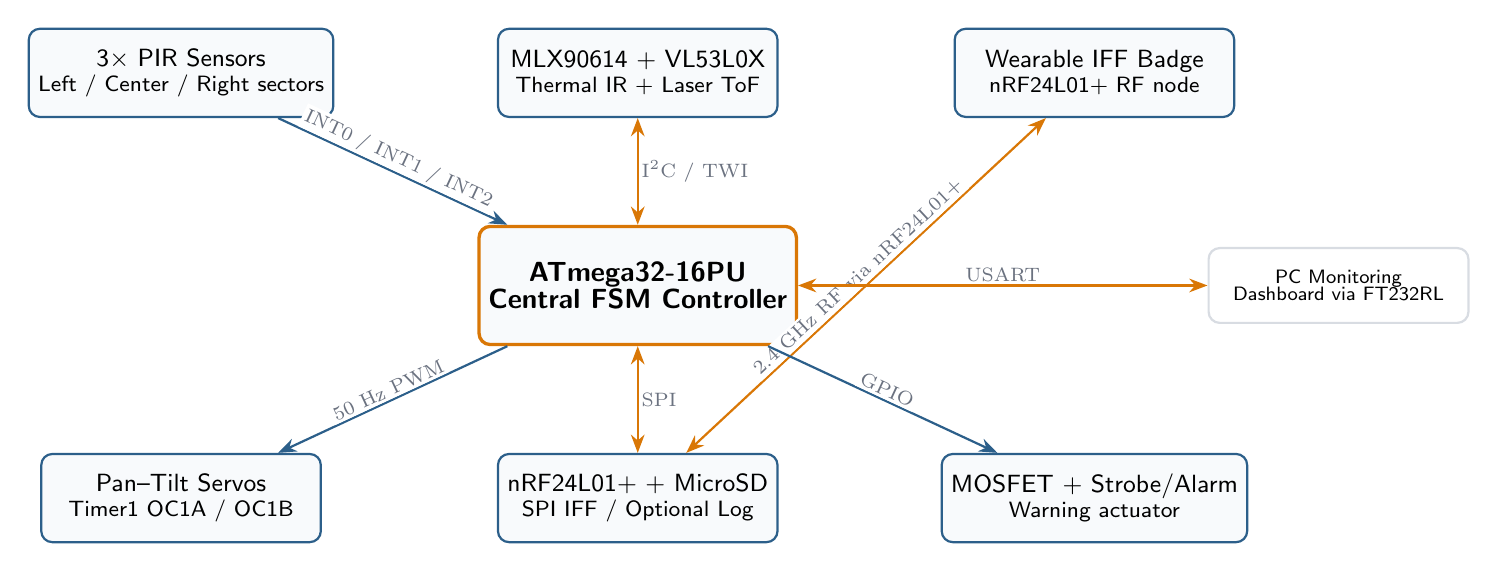
\begin{tikzpicture}[
            mcu/.style={rectangle, draw=AmberAccent, very thick, fill=CardBg, rounded corners, minimum height=1.5cm, minimum width=3.8cm, align=center, font=\sffamily\bfseries\normalsize},
            block/.style={rectangle, draw=TealAccent, thick, fill=CardBg, rounded corners, minimum height=1.12cm, minimum width=3.55cm, align=center, font=\sffamily\small},
            smallblock/.style={rectangle, draw=Line, thick, fill=white, rounded corners, minimum height=0.95cm, minimum width=3.3cm, align=center, font=\sffamily\scriptsize},
            arrow/.style={-Stealth, thick, color=TealAccent},
            biarrow/.style={Stealth-Stealth, thick, color=AmberAccent},
            lbl/.style={font=\scriptsize, color=TextDim, fill=white, inner sep=1pt}
        ]
            % Sensing layer
            \node[block] (pir) at (-5.8,2.7) {3$\times$ PIR Sensors\\[-2pt]\footnotesize Left / Center / Right sectors};
            \node[block] (thermal) at (0,2.7) {MLX90614 + VL53L0X\\[-2pt]\footnotesize Thermal IR + Laser ToF};
            \node[block] (badge) at (5.8,2.7) {Wearable IFF Badge\\[-2pt]\footnotesize nRF24L01+ RF node};

            % Central controller
            \node[mcu] (mcu) at (0,0) {ATmega32-16PU\\[-2pt]\normalsize Central FSM Controller};

            % Output layer
            \node[block] (servo) at (-5.8,-2.7) {Pan--Tilt Servos\\[-2pt]\footnotesize Timer1 OC1A / OC1B};
            \node[block] (wireless) at (0,-2.7) {nRF24L01+ + MicroSD\\[-2pt]\footnotesize SPI IFF / Optional Log};
            \node[block] (warning) at (5.8,-2.7) {MOSFET + Strobe/Alarm\\[-2pt]\footnotesize Warning actuator};

            % Optional PC
            \node[smallblock] (pc) at (8.9,0) {PC Monitoring\\[-2pt] Dashboard via FT232RL};

            % Connections
            \draw[arrow] (pir) -- node[lbl, above, sloped]{INT0 / INT1 / INT2} (mcu);
            \draw[biarrow] (thermal) -- node[lbl, right]{I$^2$C / TWI} (mcu);
            \draw[biarrow] (badge) -- node[lbl, above, sloped]{2.4 GHz RF via nRF24L01+} (wireless);
            \draw[arrow] (mcu) -- node[lbl, above, sloped]{50 Hz PWM} (servo);
            \draw[biarrow] (mcu) -- node[lbl, right]{SPI} (wireless);
            \draw[arrow] (mcu) -- node[lbl, above, sloped]{GPIO} (warning);
            \draw[biarrow] (mcu) -- node[lbl, above]{USART} (pc);
        \end{tikzpicture}
    }
    \vspace{0.1cm}

    {\tiny\color{TextDim} $\rightarrow$ one-way control/signal path \quad $\leftrightarrow$ bidirectional/shared communication path. HC-SR04, LCD, and battery ADC monitoring are intentionally removed for consistency.}
\end{frame}

% --- SLIDE 8: SYSTEM DESIGN - PINOUT MAP ---
\begin{frame}{3. System Design}{ATmega32 Interface Pinout Allocation Map}
    \scriptsize
    \begin{table}
        \centering
        \begin{tabular}{lll}
            \toprule
            \textbf{\color{Accent} Pin(s)} & \textbf{\color{Accent} Function} & \textbf{\color{Accent} Connected To} \\
            \midrule
            PD0 (RXD), PD1 (TXD) & Hardware USART & FTDI FT232RL, 115200 baud \\
            PD2 (INT0) & External interrupt 0 & Left sector PIR trigger \\
            PD3 (INT1) & External interrupt 1 & Center sector PIR trigger \\
            PB2 (INT2) & External interrupt 2 & Right sector PIR trigger \\
            PD5 (OC1A) & Timer1 hardware PWM & Pan servo control signal \\
            PD4 (OC1B) & Timer1 hardware PWM & Tilt servo control signal \\
            PC0 (SCL), PC1 (SDA) & Hardware TWI (I$^2$C) & MLX90614 and VL53L0X, 7-bit addresses 0x5A and 0x29 \\
            PB5/PB6/PB7 & Hardware SPI & MOSI / MISO / SCK for nRF24L01+ and MicroSD \\
            PB4 (SS) & SPI master safety pin & Configure as output and keep HIGH \\
            PA1 & GPIO output & MicroSD chip select (CS\_SD) \\
            PA2 & GPIO output & nRF24L01+ CSN \\
            PA3 & GPIO output & nRF24L01+ CE \\
            PA4 & GPIO input, optional & nRF24L01+ IRQ \\
            PD6 & GPIO output & Warning strobe/alarm MOSFET gate \\
            \bottomrule
        \end{tabular}
    \end{table}
\end{frame}

% --- SLIDE 9: ROLE OF THE ATMEGA32 - FSM ---
\begin{frame}{4. Role of the ATmega32}{Finite State Machine Logic}
    \centering
    \vspace{0.15cm}
    \resizebox{0.92\textwidth}{!}{
        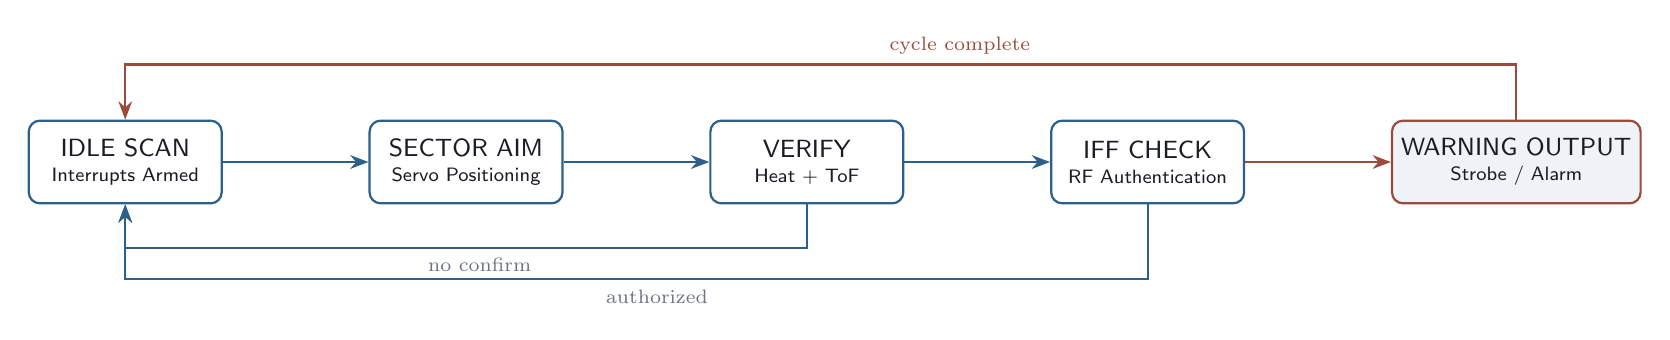
\begin{tikzpicture}[
            node distance=1.85cm,
            state/.style={
                rectangle,
                draw=Accent,
                fill=white,
                thick,
                rounded corners,
                minimum height=1.05cm,
                minimum width=2.45cm,
                align=center,
                font=\sffamily\small,
                text=Ink
            },
            alertstate/.style={
                state,
                draw=Warn,
                fill=AccentSoft
            },
            arrow/.style={-Stealth, thick, color=Accent},
            alertarrow/.style={-Stealth, thick, color=Warn},
            note/.style={font=\scriptsize, color=Dim}
        ]
            \node[state] (idle) {IDLE SCAN\\[-2pt]\scriptsize Interrupts Armed};
            \node[state, right=of idle] (aim) {SECTOR AIM\\[-2pt]\scriptsize Servo Positioning};
            \node[state, right=of aim] (verify) {VERIFY\\[-2pt]\scriptsize Heat + ToF};
            \node[state, right=of verify] (iff) {IFF CHECK\\[-2pt]\scriptsize RF Authentication};
            \node[alertstate, right=of iff] (warn) {WARNING OUTPUT\\[-2pt]\scriptsize Strobe / Alarm};

            % Main forward flow
            \draw[arrow] (idle) -- (aim);
            \draw[arrow] (aim) -- (verify);
            \draw[arrow] (verify) -- (iff);
            \draw[alertarrow] (iff) -- (warn);

            % Feedback / return paths
            \draw[arrow] (verify.south) -- ++(0,-0.55) -| node[pos=0.24, below, note]{no confirm} (idle.south);
            \draw[arrow] (iff.south) -- ++(0,-0.95) -| node[pos=0.24, below, note]{authorized} (idle.south);
            \draw[alertarrow] (warn.north) -- ++(0,0.70) -| node[pos=0.20, above, note, text=Warn]{cycle complete} (idle.north);
        \end{tikzpicture}
    }

    \vspace{0.30cm}
    \begin{itemize}
        \small
        \item The FSM proceeds through sector detection, servo aiming, thermal/range verification, IFF check, and warning output.
        \item Feedback paths return the controller to \textbf{IDLE SCAN} when the target is not confirmed, the IFF is authorized, or the warning cycle completes.
    \end{itemize}
\end{frame}

% --- SLIDE 10: ROLE OF THE ATMEGA32 - PERIPHERAL UTILIZATION ---
\begin{frame}{4. Role of the ATmega32}{Peripheral Utilization Breakdown}
    \footnotesize
    \begin{itemize}
        \item \textbf{GPIO:} warning MOSFET control, status indicators, SPI chip-select/control lines.
        \item \textbf{External interrupts (INT0/1/2):} low-latency sector detection from three PIR sensors.
        \item \textbf{Timer1 (16-bit):} exact 50 Hz servo PWM using OC1A and OC1B for pan and tilt.
        \item \textbf{Timer0:} 1 ms system tick for non-blocking task scheduling and state-machine timing.
        \item \textbf{Timer2:} spare timer for optional timeout generation or future buzzer output.
        \item \textbf{Hardware TWI (I$^2$C):} 100 kHz bus to MLX90614 and VL53L0X.
        \item \textbf{Hardware SPI:} master mode, shared by nRF24L01+ and optional MicroSD using separate CS/CSN lines.
        \item \textbf{Hardware USART:} 115200 baud telemetry frames, e.g. \texttt{\$SECTOR,DIST,TEMP,STATUS\#}.
    \end{itemize}
\end{frame}

% --- SLIDE 11: IMPLEMENTATION PLAN - MILESTONES ---
\begin{frame}{5. Implementation Plan}{Milestones}
    \begin{columns}[T]
        \begin{column}{0.48\textwidth}
            \begin{block}{Project Update 1 (Wks 1--3)}
                \footnotesize
                \begin{itemize}
                    \item 1.1 Bare-metal clock, GPIO, and register setup
                    \item 1.2 Timer1 50 Hz PWM for pan-tilt servos
                    \item 1.3 Hardware I$^2$C driver: MLX90614 + VL53L0X
                    \item 1.4 External interrupts for three-sector PIR detection
                \end{itemize}
                \textbf{Deliverable:} turret aims to activated sector and sends distance/temperature over UART.
            \end{block}
        \end{column}
        \begin{column}{0.48\textwidth}
            \begin{block}{Final Demonstration (Wks 4--6)}
                \footnotesize
                \begin{itemize}
                    \item 2.1 SPI driver for nRF24L01+ and optional MicroSD logging
                    \item 2.2 Application-layer IFF challenge-response handshake
                    \item 2.3 PC monitoring dashboard over UART
                    \item 2.4 MOSFET-driven strobe/alarm warning output
                    \item 2.5 Power isolation, level shifting, enclosure, and stress testing
                \end{itemize}
                \textbf{Deliverable:} sector detection, servo aiming, thermal/range verification, IFF, warning output, and dashboard.
            \end{block}
        \end{column}
    \end{columns}
\end{frame}

% --- SLIDE 12: IMPLEMENTATION PLAN - TEAM RESPONSIBILITIES ---
\begin{frame}{5. Implementation Plan}{Group Member Responsibilities}
    \begin{columns}[T]
        \begin{column}{0.32\textwidth}
            \begin{block}{Member 1: Firmware \& Control}
                \small
                \begin{itemize}
                    \item Register-level drivers: GPIO, Timer1 PWM, Timer0 tick, I$^2$C, external interrupts
                    \item Core FSM architecture
                    \item Timing-loop optimization
                \end{itemize}
            \end{block}
        \end{column}
        \begin{column}{0.32\textwidth}
            \begin{block}{Member 2: Hardware, Power \& Actuation}
                \small
                \begin{itemize}
                    \item Pan-tilt turret assembly
                    \item 5 V/6 V power distribution and decoupling
                    \item Sensor calibration, level shifting, MOSFET warning circuit
                \end{itemize}
            \end{block}
        \end{column}
        \begin{column}{0.32\textwidth}
            \begin{block}{Member 3: Wireless, Storage \& GUI}
                \small
                \begin{itemize}
                    \item SPI management for nRF24L01+ and optional MicroSD
                    \item IFF challenge-response protocol logic
                    \item Python monitoring dashboard
                \end{itemize}
            \end{block}
        \end{column}
    \end{columns}
\end{frame}

% --- SLIDE 13: USE OF OTHER CONTROLLERS ---
\begin{frame}{6. Use of Other Controllers}{Required Auxiliary IFF Badge}
    \begin{block}{Main System}
        \small The ATmega32 is the sole main controller. It handles the fixed station: PIR detection, servo aiming, sensor verification, RF challenge initiation, optional logging, UART dashboard, and warning output.
    \end{block}
    \begin{block}{Auxiliary Controller -- Wearable IFF Badge}
        \small
        \begin{itemize}
            \item \textbf{Device:} Arduino Nano / ATtiny85, battery-powered and worn by authorized personnel.
            \item \textbf{Why required:} the badge is physically separate from the fixed turret station, so it needs its own small controller.
            \item \textbf{Task:} receives a 2.4 GHz challenge packet and returns a keyed response using its own nRF24L01+ module.
            \item \textbf{Interface:} wireless RF only; it performs no main-system sensing, aiming, logging, or warning-output tasks.
        \end{itemize}
    \end{block}
\end{frame}

% --- SLIDE 14: TESTING AND SUCCESS CRITERIA ---
\begin{frame}{7. Testing \& Success Criteria}{Measurable Criteria \& Test Methodology}
    \scriptsize
    \begin{table}
        \centering
        \begin{tabular}{llll}
            \toprule
            \textbf{\color{Accent} Metric} & \textbf{\color{Accent} Target} & \textbf{\color{Accent} Test Method} & \textbf{\color{Accent} Priority} \\
            \midrule
            Sector detection latency & $< 100$ ms & PIR trigger to MCU state change & Essential \\
            Turret slew speed & $< 500$ ms & Trigger-to-sector-angle timing & Essential \\
            Servo PWM stability & 50 Hz on OC1A/OC1B & Oscilloscope waveform check & Essential \\
            Distance verification & $\pm 30$ mm, 10--120 cm & VL53L0X indoor matte-target bench test & Essential \\
            Thermal verification & $\Delta T \ge 3^\circ$C above background & Controlled warm-object test & Essential \\
            I$^2$C bus stability & Clean SCL @ 100 kHz & Multi-device signal-integrity check & Essential \\
            IFF handshake execution & $< 50$ ms & RF challenge-response timing & Essential \\
            Warning output & Correct MOSFET switching & Strobe/alarm activation test & Essential \\
            Telemetry streaming rate & $\ge 10$ Hz, no frame loss & PC dashboard continuous update & Optional \\
            MicroSD black-box log & Event timestamp/sector/heat/range & File readback verification & Optional \\
            \bottomrule
        \end{tabular}
    \end{table}
    \vspace{0.15cm}
    \footnotesize\color{Dim} Essential features: PIR sector detection, Timer1 servo aiming, I$^2$C heat/range verification, IFF handshake, and warning output. Optional features: MicroSD logging and PC monitoring dashboard.
\end{frame}

% --- SLIDE 15: CHALLENGES AND FUTURE SCOPE ---
\begin{frame}{8. Challenges \& Future Scope}{Anticipated Issues \& Scaling Path}
    \begin{columns}[T]
        \begin{column}{0.48\textwidth}
            \begin{block}{Technical \& Hardware Challenges}
                \footnotesize
                \begin{itemize}
                    \item \textbf{SPI sharing:} nRF24L01+ needs low-latency packets while MicroSD performs longer writes $\rightarrow$ separate CS lines and bus-release routines.
                    \item \textbf{3.3 V modules:} VL53L0X and nRF24L01+ require correct regulation/level compatibility $\rightarrow$ level shifting or safe breakout boards.
                    \item \textbf{Servo noise:} high current spikes can reset the MCU $\rightarrow$ isolated servo rail, common ground, and bulk decoupling.
                    \item \textbf{Sensor certainty:} MLX90614 confirms a warm object, not identity $\rightarrow$ combine heat, range, sector, and IFF results.
                \end{itemize}
            \end{block}
        \end{column}
        \begin{column}{0.48\textwidth}
            \begin{block}{Future Scope}
                \footnotesize
                \begin{itemize}
                    \item \textbf{Computer vision:} ESP32-CAM co-processor for visual target classification.
                    \item \textbf{360$^\circ$ coverage:} stepper/continuous-rotation mechanism with slip ring support.
                    \item \textbf{Long-range communication:} LoRa telemetry network for multi-unit perimeter monitoring.
                \end{itemize}
            \end{block}
        \end{column}
    \end{columns}
\end{frame}

\end{document}
